\documentclass[twocolumn,10pt]{article}
\title{Area and circumference of circles}
\setlength{\columnsep}{20pt} 
\usepackage{amsmath,hyperref,cancel,graphicx}
 \def\shrinkfactor{0.45}
 \usepackage[margin=1.5cm]{geometry}
\usepackage[usenames,dvipsnames]{color}
 
 \newcommand{\blue}[1]{{\color{Blue}#1}} 
 \newcommand{\purple}[1]{{\color{Purple}#1}} 
 \newcommand{\red}[1]{{\color{Red}#1}} 
 \newcommand{\green}[1]{{\color{Green}#1}} 
 \newcommand{\gray}[1]{{\color{Gray}#1}} 
  \newcommand{\pink}[1]{{\color{Magenta}#1}}   
\RequirePackage[normalem]{ulem} \RequirePackage{color}\definecolor{RED}{rgb}{1,0,0}\definecolor{BLUE}{rgb}{0,0,1} \providecommand{\DIFadd}[1]{{\protect\color{blue}\uwave{#1}}} \providecommand{\DIFdel}[1]{{\protect\color{red}\sout{#1}}}                      \providecommand{\DIFaddbegin}{} \providecommand{\DIFaddend}{} \providecommand{\DIFdelbegin}{} \providecommand{\DIFdelend}{} \providecommand{\DIFaddFL}[1]{\DIFadd{#1}} \providecommand{\DIFdelFL}[1]{\DIFdel{#1}} \providecommand{\DIFaddbeginFL}{} \providecommand{\DIFaddendFL}{} \providecommand{\DIFdelbeginFL}{} \providecommand{\DIFdelendFL}{} 
\begin{document}
\maketitle



\DIFdelbegin 
\DIFdelend \section{\href{https://www.khanacademy.org/devadmin/content/items/x16ef58f4aa84f33e}{x16ef58f4aa84f33e}}

\noindent
While visiting the moon, you \DIFdelbegin \DIFdel{are come to }\DIFdelend \DIFaddbegin \DIFadd{encounter }\DIFaddend a huge circular crater. You want to measure the area of the crater. You decide to walk around the perimeter of the crater and measure its circumference.

**If the circumference is $C=6\pi\text{ km}$, what is the area of the crater?**


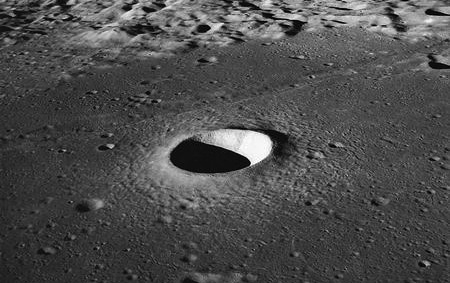
\includegraphics[scale=\shrinkfactor]{figures/bd11fceae4eea83cbcc716bef8625a79765f78fc.jpeg}


\paragraph{Ans} $A=$ [[? input-number 1]]  $\text{ km}$  28.274333882308138

\paragraph{Hint 1}This problem requires us to use both the formula of the circumference of a circle $\blue{C}=2\pi \red{r}$, and the formula for the area of a circle $\purple{A}=\pi \red{r}^2$, 

\paragraph{Hint 2}You measured the length of the circumference of the crater to be $\blue{C} =\blue{6\pi}\text{ km}$.

To find the radius of the crater, we solve for $\red{r}$ in the following equation 

\begin{align*}
  \qquad  2\pi \red{r} &= \blue{C} \\[1mm]
2\pi \red{r} 	&= \blue{6\pi}\text{ km} \\[1mm]
 2\cancel{\pi} \red{r} 	
&= 6\cancel{\pi}\text{ km} \\[1mm] 
  \red{r} &= \red{3}\text{ km}
\end{align*}

\paragraph{Hint 3}We can now plug the radius $\red{r} = \red{3}\text{ km}$ in to the area formula to obtain:

\begin{align*}
  \qquad  \purple{A} &= \pi \red{r}^2 \\[1mm]
  &= \pi(\red{3} \text{ km})^2  \\[1mm]
 &= \purple{9\pi} \text{ km}^2
\end{align*}

\paragraph{Hint 4}The area of the crater is $9\pi \text{ km}^2$.



\medskip
\noindent
\textbf{Tags:} {\footnotesize CC.7.G.B.4, SB.7.1.F.2.SR, Area and circumference of a circle.circle area, Area and circumference of a circle.Circle circumference}\\
\textbf{Version:} \DIFdelbegin \DIFdel{1573aeac.. 2013-10-15
}\DIFdelend \DIFaddbegin \DIFadd{965adae5.. 2013-10-16
}\DIFaddend \smallskip\hrule





\section{\href{https://www.khanacademy.org/devadmin/content/items/x207f8a7e9a127fad}{x207f8a7e9a127fad}}

\noindent
An engineer is planning a new water pipe installation.
The pipe has a diameter of $d=20\text{ cm}$.

**What is the area of the cross section of this pipe?**

\paragraph{Ans} $A =$ [[? input-number 1]] $\text{cm}^2$        314.1592653589793

\paragraph{Hint 1}This problem calls for the formula for the area of a circle $\purple{A} = \pi \red{r}^2$.


\paragraph{Hint 2}The diameter of the pipe is $\green{d}=\green{20}\text{ cm}$. Since the diameter of a circle is double the length of the radius, the radius of the pipe is $\red{r}=\frac{\green{d}}{2} = \red{10}\text{ cm}$.

\paragraph{Hint 3}We can now use the formula for the area of a circle $\purple{A} = \pi \red{r}^2$ to calculate the area of the pipe. The area of a pipe with radius $\red{r}=\red{10}\text{ cm}$ is

\begin{align*}
  \qquad \purple{A}  	&= \pi \red{r}^2 				\\
  		&= \pi (\red{10})^2			\\
  		&= \pi (100)		\\
  		&= 100 \pi \text{ cm}^2
\end{align*}

\paragraph{Hint 4}The area of the cross section of this pipe is $100\pi  \text{ cm}^2$. 



\medskip
\noindent
\textbf{Tags:} {\footnotesize CC.7.G.B.4, SB.7.1.F.2.SR, Area and circumference of a circle.circle area}\\
\textbf{Version:} 975543c7.. 2013-09-29
\smallskip\hrule





\section{\href{https://www.khanacademy.org/devadmin/content/items/x3879b8b46e93651e}{x3879b8b46e93651e}}

\noindent
A baker uses a coffee mug with diameter $d=8\text{ cm}$  to cut out circular cookies from a big sheet of cookie dough.  

**What is the area of each cookie?**

\paragraph{Ans} $A=$ [[? input-number 1]] $\text{cm}^2$  50.26548245743669

\paragraph{Hint 1}This problem calls for the formula for the area of a circle $\purple{A}=\pi \red{r}^2$. 

\paragraph{Hint 2}The cup has a circular shape and its diameter is $\green{d}=\green{8}\text{ cm}$.

The radius of the cup is 

$\qquad \red{r} = \dfrac{\green{d}}{2}= \dfrac{\green{8}\text{ cm}}{2}=\red{4}\text{ cm}$.

To find the area, we substitute the value $\red{r} = \red{4}\text{ cm}$ into the formula for the area of a circle.

\paragraph{Hint 3}Using the formula  $\purple{A}=\pi \red{r}^2$, we find the area of each cookie is

\begin{align*}
 \qquad \purple{A} 	& =\pi \red{r}^2 	\\
  	& = \pi (\red{4}\text{ cm})^2		\\
  	& = \pi (\red{4} \times \red{4}) \text{ cm}^2		\\
  	&= 16 \pi  \text{ cm}^2		
\end{align*}

The area of each cookie is  $16 \pi \text{ cm}^2$.



\medskip
\noindent
\textbf{Tags:} {\footnotesize CC.7.G.B.4, SB.7.1.F.2.SR, Area and circumference of a circle.circle area}\\
\textbf{Version:} dfcce67c.. 2013-10-09
\smallskip\hrule





\section{\href{https://www.khanacademy.org/devadmin/content/items/x46f48b406167b396}{x46f48b406167b396}}

\noindent
While visiting the moon, you come to a huge crater. You know the area of this crater is $A=9\pi\text{ km}^2$. 

**What is the circumference of the crater?**


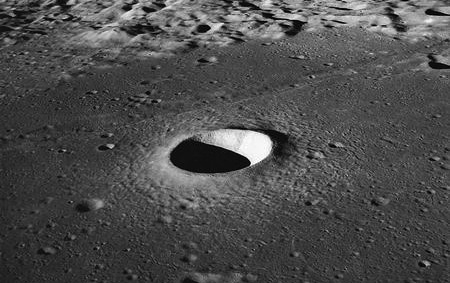
\includegraphics[scale=\shrinkfactor]{figures/bd11fceae4eea83cbcc716bef8625a79765f78fc.jpeg}


\paragraph{Ans} $C=$ [[? input-number 1]]  $\text{ km}$  18.84955592153876

\paragraph{Hint 1}This problem requires us to use both the formula of the circumference of a circle $\blue{C}=2\pi \red{r}$, and the formula for the area of a circle $\purple{A}=\pi \red{r}^2$, 

\paragraph{Hint 2}You know the area of the crater is $\purple{A} =\purple{9\pi}\text{ km}^2$.

To find the radius of the crater, we solve for $\red{r}$ in the following equation 

\begin{align*}
\qquad \pi \red{r}^2   &= \purple{9\pi} \text{ km}^2  \\[1mm]
\cancel{\pi} \red{r}^2   &= 9\cancel{\pi} \text{ km}^2  \\[1mm] 
\red{r}^2 &= 9\text{ km}^2 \\[1mm]
\red{r} &= 3\text{ km} \\[1mm]
\end{align*}


Note the reasoning we used in the last step: $\red{r}^2=9=3\cdot3=3^2$, therefore $\red{r}=\red{3}$.  Since the area is measured in $\text{km}^2$ the radius is measured in $\text{km}$.

\paragraph{Hint 3}We can now plug the radius $\red{r} = \red{3}\text{ km}$ in to the circumference formula to obtain

\begin{align*}
  \qquad \blue{C}  &= 2\pi \red{r}  \\[1mm]
&= 2\pi (\red{3}\text{ km})  \\[1mm]
&= \blue{6\pi}\text{ km}
\end{align*}

\paragraph{Hint 4}The circumference of the crater is $6\pi \text{ km}$.



\medskip
\noindent
\textbf{Tags:} {\footnotesize CC.7.G.B.4, SB.7.1.F.2.SR, Area and circumference of a circle.circle area, Area and circumference of a circle.Circle circumference}\\
\textbf{Version:} b985a584.. 2013-10-15
\smallskip\hrule





\section{\href{https://www.khanacademy.org/devadmin/content/items/x4d9ac4ed5246f99b}{x4d9ac4ed5246f99b}}

\noindent
Your local pizza place offers the following two pizza deals, both for the same price:   
Option 1: One extra-large pizza with diameter $20\text{ in}$.  
Option 2: Two medium pizzas with diameter $15\text{ in}$ each.

**Which of the options offers a bigger area of pizza?**


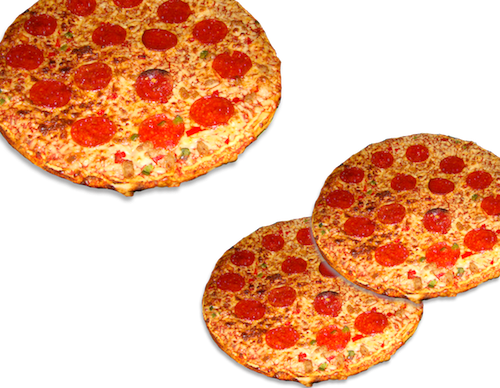
\includegraphics[scale=\shrinkfactor]{figures/5ac1d9f5c91daf1f9f7c2bcb006c279c70abc72a.png}


\paragraph{Ans} Option 1 offers a total pizza area of  [[? input-number 1]]$\text{ in}^2$  while Option 2 offers an area of [[? input-number 2]]$\text{ in}^2$, so [[? dropdown 1]] has a lower price per square inch.  314.1592653589793

\paragraph{Hint 1}Let's use the area formula $\purple{A}=\pi \red{r}^2$ to find the area of pizza for the two deals.

\paragraph{Hint 2}For Option 1, the total area of pizza is equal to the area of the extra-large pizza 

\begin{align*}
\qquad A_1 
  &= A_{\text{extra-large}}  \\
  &= \pi \red{r}^2  \\
  & = \pi (\red{10})^2  \\
  &= \pi 100 \text{ in}^2
\end{align*}

\paragraph{Hint 3}For Option 2, the total area of pizza is the sum of the areas of the two medium pizzas

\begin{align*}
\qquad A_2 
 &= \blue{2}A_{\text{medium}} \\
  &= \blue{2}\left[\pi \red{r}^2 \right] \\
 &= \blue{2}\left[\pi (\red{7.5})^2\right]  \\
 &= \blue{2}\left[\pi \left(\red{\frac{15}{2}}\right)^2\right]  \\
 &= \blue{2}\left[\pi  \frac{225}{4} \right]  \\
 &= \frac{225\pi}{2}\text{ in}^2
\end{align*}

\paragraph{Hint 4}Option 1 offers a total pizza area of $ 100\pi \text{ in}^2$ while the area of Option 2 is \DIFdelbegin \DIFdel{$\frac{225}{2}\text{ in}^2$}\DIFdelend \DIFaddbegin \DIFadd{$\frac{225}{2}\pi\text{ in}^2$}\DIFaddend .

Since $\frac{225}{2} > 100$, **Option 2** has a lower price per square inch of pizza.



\medskip
\noindent
\textbf{Tags:} {\footnotesize CC.7.G.B.4, SB.7.1.F.2.SR, Area and circumference of a circle.circle area}\\
\textbf{Version:} \DIFdelbegin \DIFdel{dac9305e.. 2013-10-15
}\DIFdelend \DIFaddbegin \DIFadd{0ae227ad.. 2013-10-16
}\DIFaddend \smallskip\hrule





\section{\href{https://www.khanacademy.org/devadmin/content/items/x53718caed7c5f72f}{x53718caed7c5f72f}}

\noindent
If the radius of a circle is multiplied by a factor of $3$, by what factor will the area of the circle increase?

\paragraph{Ans} The area of a circle with radius $3$ is [[? input-number 1]] times bigger than the area of a circle with radius $1$.  9

\paragraph{Hint 1}Let's look at the formula for the area of a circle $A=\pi r^2$.  

How will the area change if we the radius is tripled?

\paragraph{Hint 2}The area of a circle of radius $r=a$ is $\pi a^2$.

The area of a circle with radius $r=3a$ is 

\begin{align*}
\qquad 
 \pi r^2 & =\pi (3a)^2  \\
  & =\pi(3a)(3a) \\
  &=\pi(3 \times 3 \times a \times a)  \\
   &= \pi \times 9 \times a^2 \\
   &= 9\pi a^2,
\end{align*} 

which is $9$ times bigger than the area of a circle of radius $r=a$. 

\paragraph{Hint 3}When the radius of a circle is tripled, the area increases $9$ times because the radius $r$ is squared in the formula $A=\pi r^2$. 



\medskip
\noindent
\textbf{Tags:} {\footnotesize CC.7.G.B.4, SB.7.1.F.2.SR, Area and circumference of a circle.circle area}\\
\textbf{Version:} 7c11a267.. 2013-10-11
\smallskip\hrule





\section{\href{https://www.khanacademy.org/devadmin/content/items/x96a8cbf4fb017d88}{x96a8cbf4fb017d88}}

\noindent
A compact-disk (CD) has a diameter of $12\text{ cm}$. The hole in the middle has a diameter of $1.5\text{ cm}$. 

**What is the area of the disk?**  


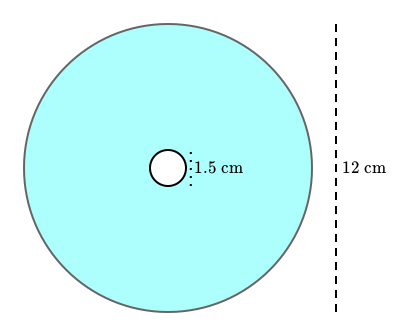
\includegraphics[scale=\shrinkfactor]{figures/fea5db7586f0e819785c674bb2fc6212dda1ce88.png}

\paragraph{Ans} $A =$ [[? input-number 1]] $\text{cm}^2$  111.33018966158829

\paragraph{Hint 1}The area of a CD is equal to the total area the disk minus the area of the hole in the middle.

\paragraph{Hint 2}We need to use the formula for the area of a circle $\purple{A} = \pi \red{r}^2$ two times.

The outer radius of the disk is $\red{r} = \frac{\green{d}}{2}=\frac{\green{12}\text{ cm}}{2}=\red{6}\text{ cm}$, so the area of the disk (including the hole) is   

\begin{align*}
  \qquad \purple{A}_{\text{outer}}  	&= \pi \red{r}^2 			\\
  		&= \pi (\red{6}\text{ cm})^2			\\
  		&= \pi (\red{6} \times \red{6}) \text{ cm}^2			\\
  		&= 36 \pi  \text{ cm}^2		
\end{align*}


\paragraph{Hint 3}The radius of the hole in the middle is $\red{r} = \frac{\green{d}}{2}= \frac{\green{1.5}\text{ cm}}{2}=\red{0.75}\text{ cm}$, so the area of the hole is

\begin{align*}
  \qquad \purple{A}_{\text{hole}}  	&= \pi \red{r}^2 				\\
  		&= \pi (\red{0.75}\text{ cm})^2			\\
  		&= \pi (\red{0.75} \times \red{0.75}) \text{ cm}^2			\\
  		&= \pi \left(\red{\frac{3}{4}} \times \red{\frac{3}{4}}\right) \text{ cm}^2			\\
  		&= \frac{9\pi}{16} \text{ cm}^2		
\end{align*}

\paragraph{Hint 4}The area of the CD is  

\DIFdelbegin \begin{eqnarray*}\DIFdel{
\quad \purple{A}_{\text{CD}} 
  }&\DIFdel{= \purple{A}_{\text{outer}} - \purple{A}_{\text{hole}} }\\[2mm] 
  &\DIFdel{= 36\pi -  \frac{9\pi}{16}  }\\[1.2mm]
  &\DIFdel{= \left(36 -  \frac{9}{16}\right)\pi  }\\[1.2mm]
  &\DIFdel{= \left(\frac{36\times\blue{16}}{\blue{16}} -  \frac{9}{16}\right)\pi  }\\[1.2mm]
  &\DIFdel{= \left(\frac{576}{16} -  \frac{9}{16}\right)\pi  }\\[1.2mm]
  &\DIFdel{= \frac{567\pi}{16} \text{ cm}^2.
}\end{eqnarray*}
\DIFdelend \DIFaddbegin \begin{align*}\DIFadd{
\quad \purple{A}_{\text{CD}} 
  }&\DIFadd{= \purple{A}_{\text{outer}} - \purple{A}_{\text{hole}} }\\[2mm] 
  &\DIFadd{= 36\pi -  \frac{9\pi}{16}  }\\[1.2mm]
  &\DIFadd{= \left(36 -  \frac{9}{16}\right)\pi  }\\[1.2mm]
  &\DIFadd{= \left(\frac{36\times\blue{16}}{\blue{16}} -  \frac{9}{16}\right)\pi  }\\[1.2mm]
  &\DIFadd{= \left(\frac{576}{16} -  \frac{9}{16}\right)\pi  }\\[1.2mm]
  &\DIFadd{= \frac{567\pi}{16} \text{ cm}^2
}\end{align*}
\DIFaddend 

\paragraph{Hint 5}We obtain the final answer $A_{\text{CD}}=\frac{567\pi}{16}\text{ cm}^2$, which is approximately equal to $111.3\text{ cm}^2$.



\medskip
\noindent
\textbf{Tags:} {\footnotesize CC.7.G.B.4, SB.7.1.F.2.SR, Area and circumference of a circle.circle area}\\
\textbf{Version:} \DIFdelbegin \DIFdel{75e8b0f9.. 2013-10-11
}\DIFdelend \DIFaddbegin \DIFadd{1d4644d5.. 2013-10-16
}\DIFaddend \smallskip\hrule





\section{\href{https://www.khanacademy.org/devadmin/content/items/xa9879653bc4a66ea}{xa9879653bc4a66ea}}

\noindent
When the radius of a circle is multiplied by a factor of $2$, by what factor will the area of the circle increase?

\paragraph{Ans} The area of a circle with radius $2$ is [[? input-number 1]] times bigger than the area of a circle with radius $1$.  4

\paragraph{Hint 1}Let's look at the formula for the area of a circle $A=\pi r^2$. 

How will the area change if the radius doubles?

\paragraph{Hint 2}The area of a circle of radius $r=a$ is $\pi a^2$.

The area of a circle with radius $r=2a$ is 

\begin{align*}
\qquad  \pi r^2 & =\pi (2a)^2  \\
  & =\pi(2a)(2a) \\
  &=\pi(2 \times 2 \times a \times a)  \\
   &= \pi \times 4 \times a^2 \\
   &= 4\pi a^2,
\end{align*} 

which is $4$ times bigger than the area of a circle of radius $r=a$. 

\paragraph{Hint 3}When the radius of a circle doubles, the area increases $4$ times because the radius $r$ is squared in the formula $A=\pi r^2$.




\medskip
\noindent
\textbf{Tags:} {\footnotesize CC.7.G.B.4, SB.7.1.F.2.SR, Area and circumference of a circle.circle area}\\
\textbf{Version:} a3412e12.. 2013-10-09
\smallskip\hrule





\section{\href{https://www.khanacademy.org/devadmin/content/items/xc36d0fcab2738fb5}{xc36d0fcab2738fb5}}

\noindent
A building engineer is analyzing a concrete column which has a circular cross section. 
The circumference of the column is $C =18 \pi\text{ m}$. 

**What is the area of the cross section of the column?**

State your answer in \DIFaddbegin \DIFadd{$\text{m}^2$}\DIFaddend .

\paragraph{Ans} $A =$ [[? input-number 1]] $\text{ m}^2$  254.46900494077323

\paragraph{Hint 1}The cross section of the concrete column is a circle. The engineer knows the circumference of the circle and wants to find the area. 

We must combine the formulas $\blue{C}=2\pi \red{r}$ and $\purple{A}=\pi \red{r}^2$ to solve this problem.


\paragraph{Hint 2}The circumference of a circle with radius $\red{r}$ is $\blue{C}=2\pi \red{r}$. 
Since we know $\blue{C}=\blue{18\pi}\text{ m}$, we can find $\red{r}$ by solving the following equation:

\begin{align*}
   \qquad 2\pi \red{r} 	&= \blue{18\pi} \text{ m}	\\[1mm]
   \red{r}     	&= \dfrac{ \blue{18\pi} } { 2 \pi }  \\
   \red{r}     	&= \red{9}\text{ m}
\end{align*}

\paragraph{Hint 3}Now that we know the radius of the column is $\red{r}=\red{9}\text{ m}$, we can find the area of its cross section: 

\begin{align*}
 \qquad \purple{A} 	& =\pi \red{r}^2 					\\
& = \pi \left(\red{ 9}\right)^2	\\
& = 81\pi \text{ m}^2
\end{align*}

\paragraph{Hint 4}The area of the \DIFaddbegin \DIFadd{cross section of the }\DIFaddend concrete column is $81\pi  \text{ m}^2$.



\medskip
\noindent
\textbf{Tags:} {\footnotesize CC.7.G.B.4, SB.7.1.F.2.SR, Area and circumference of a circle.circle area, Area and circumference of a circle.Circle circumference}\\
\textbf{Version:} \DIFdelbegin \DIFdel{2dcf9729.. 2013-10-15
}\DIFdelend \DIFaddbegin \DIFadd{448adf27.. 2013-10-16
}\DIFaddend \smallskip\hrule





\section{\href{https://www.khanacademy.org/devadmin/content/items/xe448997a086976be}{xe448997a086976be}}

\noindent
An engineer is tasked to install a pipe which supplies the water to a building.
The new pipe must have a cross-sectional area of $A=100\pi \text{ cm}^2$.

**What diameter of pipe should the engineer choose?**

\paragraph{Ans} $d=$  [[? input-number 1]]  $\text{cm}$  20

\paragraph{Hint 1}This problem calls for the area formula for a circle $\purple{A} = \pi \red{r}^2$. 
We know the cross-sectional area of the pipe is  $\purple{A}=\purple{100\pi }\text{ cm}^2$
and we want to find the diameter of the pipe.

\paragraph{Hint 2}We can find the radius of the pipe if we solve for $\red{r}$ in the following equation  

\begin{align*}
 \qquad  \pi \red{r}^2  &= \purple{100\pi} \text{ cm}^2			\\
  \pi \red{r}^2 	&= 10^2\pi 			\\
   \cancel{\pi} \red{r}^2 	&= 10^2\cancel{\pi} 			\\
   \red{r}^2     			&= 10^2 				\\
   \red{r}     			&= \red{10}\text{ cm}
\end{align*}

Note the reasoning we used in the last step: $\red{r}^2=10^2$, therefore $\red{r}=\red{10}$. 
Since the area is measured in $\text{cm}^2$ the radius is measured in $\text{cm}$.

\paragraph{Hint 3}Since the diameter of the pipe is double the length of the radius, the diameter of the pipe must be $\green{d} = 2\red{r}=2(\red{10}) = \green{20}\text{ cm}$.



\medskip
\noindent
\textbf{Tags:} {\footnotesize CC.7.G.B.4, SB.7.1.F.2.SR, Area and circumference of a circle.circle area}\\
\textbf{Version:} e58edf20.. 2013-10-09
\smallskip\hrule





\section{\href{https://www.khanacademy.org/devadmin/content/items/xf793550bfea84e99}{xf793550bfea84e99}}

\noindent
You friend just pulled out a huge, home-baked pizza from the oven and tells you the area of the pizza is $A=625\pi \text{ cm}^2$.

**What \DIFaddbegin \DIFadd{is the }\DIFaddend diameter of this pizza?**


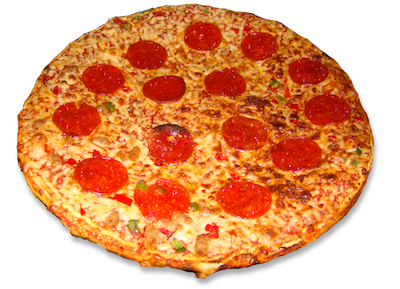
\includegraphics[scale=\shrinkfactor]{figures/1596acf0e5b2c86d980668703e3fa44c736a1635.png}

\paragraph{Ans} $d=$  [[? input-number 1]]  $\text{cm}$  50

\paragraph{Hint 1}This problem calls for the area formula of a circle $\purple{A} = \pi \red{r}^2$. 
We know the area of the pizza  is  $\purple{A}=\purple{625\pi }\text{ cm}^2$.

How do we find the diameter of the pizza?

\paragraph{Hint 2}We can find the radius of the pizza if we solve for $\red{r}$ in the following equation  

\begin{align*}
\pi \red{r}^2  &= \purple{625\pi} \text{ cm}^2			\\[2mm]
   \cancel{\pi} \red{r}^2 	&= 625\cancel{\pi}\text{ cm}^2\\
   \red{r}^2     			&= 625\text{ cm}^2
\end{align*}

To find the radius $\red{r}$ must answer the question "Which number times itself gives \DIFdelbegin \DIFdel{625}\DIFdelend \DIFaddbegin \DIFadd{$625$}\DIFaddend ?" 

The number \DIFdelbegin \DIFdel{10 is to }\DIFdelend \DIFaddbegin \DIFadd{$10$ is too }\DIFaddend small since $10\cdot10=100$, the number $20$ is also too small since $20\cdot20=400$, but $30$ is too big since $30\cdot30=900$.

The answer is $\red{r}=\red{25}\text{ cm}$ since 

$\qquad (\red{25} \text{ cm})^2=(\red{25}\cdot\red{25})\text{ cm}^2=625\text{ cm}^2$.

\paragraph{Hint 3}The diameter of the pizza is double the length of the radius  $\green{d} = 2\red{r}=2(\red{25}\text{ cm}) = \green{50}\text{ cm}$.



\medskip
\noindent
\textbf{Tags:} {\footnotesize CC.7.G.B.4, SB.7.1.F.2.SR, Area and circumference of a circle.circle area}\\
\textbf{Version:} \DIFdelbegin \DIFdel{65f6c937.. 2013-10-15
}\DIFdelend \DIFaddbegin \DIFadd{15b31456.. 2013-10-16
}\DIFaddend \smallskip\hrule





\section{\href{https://www.khanacademy.org/devadmin/content/items/x067a2ea8fceec945}{x067a2ea8fceec945}}

\noindent
A python curls up to bite the tip of its own tail forming  the shape of a circle. The python is $2.6 \pi \text{ m}$ long.  

**What is the radius of the circle it forms?**  

\paragraph{Ans} $r=$ [[? input-number 1]]  $\text{  m}$  1.3

\paragraph{Hint 1}This problem calls for the formula of the circumference of a circle $\blue{C}=2\pi \red{r}$. 

\paragraph{Hint 2}When the python curls to form the shape of a circle, the circumference of this circle is equal to the length of the python $\blue{C}=\blue{2.6\pi}\text{ m}$.

\paragraph{Hint 3}We know the formula for the circumference of a circle is $\blue{C}=2\pi \red{r}$.

If we want to find the radius of the circle formed by the python we must solve for $\red{r}$ in the following equation 

\begin{align*}
  \qquad  2\pi \red{r} 	&= \blue{2.6\pi}\text{ m} \\[1mm]
   \red{r}    &= \dfrac{ \blue{2.6\pi} } { 2 \pi }\text{ m} \\
   \red{r}     	&= \red{1.3}\text{ m}
\end{align*}


\paragraph{Hint 4}The radius of the circle formed by the python is $\red{1.3}\text{ m}$.



\medskip
\noindent
\textbf{Tags:} {\footnotesize CC.7.G.B.4, SB.7.1.F.2.SR, Area and circumference of a circle.Circle circumference}\\
\textbf{Version:} 54bf6db9.. 2013-10-15
\smallskip\hrule





\section{\href{https://www.khanacademy.org/devadmin/content/items/x1cfcca1f7e21f454}{x1cfcca1f7e21f454}}

\noindent
A wet bicycle tire leaves a trace of water on the floor. The tire has a radius of $14\text{ in}$ and the bicycle wheel makes $3$ full rotations before stopping. 

**How long is the trace of water left on the floor?**

\paragraph{Ans} [[? input-number 1]]  $\text{in}$  263.89378290154264

\paragraph{Hint 1}The length of the trace of water depends on the circumference of the tire. Each time the wheel rolls forward through one rotation, the tire leaves a mark with length equal to the circumference of the tire.

\paragraph{Hint 2}The circumference of a tire with radius $\red{r}=\red{14}\text{ in}$ is  

$\qquad \blue{C}=2\pi \red{r}=2\pi (\red{14}\text{ in})= \blue{28\pi}\text{ in}$. 

\paragraph{Hint 3}Since the bike wheel makes $\pink{3}$ full turns before stopping, the total length of the water trace is $\pink{3}$ times the circumference of the tire:  

$\qquad \text{length of water trace } = \pink{3}\times \blue{28\pi}\text{ in} = 84\pi  \text{ in}$.



\medskip
\noindent
\textbf{Tags:} {\footnotesize CC.7.G.B.4, SB.7.1.F.2.SR, Area and circumference of a circle.Circle circumference}\\
\textbf{Version:} 33f6d3d7.. 2013-09-25
\smallskip\hrule





\section{\href{https://www.khanacademy.org/devadmin/content/items/x560d92c3a06b1431}{x560d92c3a06b1431}}

\noindent
What is the ratio between a circle's circumference $C$ and its diameter $d$?


\paragraph{Ans} $\dfrac{C}{d} = $ [[? input-number 1]]   3.141592653589793

\paragraph{Hint 1}This question tests your knowledge of the formula for the circumference of a circle. 

\paragraph{Hint 2}The circumference of a circle with diameter  $\green{d}$ is given by the formula $\blue{C}=\pi \green{d}$. 

The ratio of the circle's circumference to the circle's diameter is therefore  

$\qquad \dfrac{\blue{C}}{\green{d}}=\pi$. 

\paragraph{Hint 3}In fact, this is how the number $\pi$ is defined.
The number $\pi = 3.14159265\ldots$ is defined as the ratio between the circumference and the diameter of *any* circle**.**




\medskip
\noindent
\textbf{Tags:} {\footnotesize CC.7.G.B.4, SB.7.1.F.2.SR, Area and circumference of a circle.Circle circumference}\\
\textbf{Version:} eca247ba.. 2013-10-09
\smallskip\hrule





\section{\href{https://www.khanacademy.org/devadmin/content/items/x9e0a22b47bb05fc6}{x9e0a22b47bb05fc6}}

\noindent
If the radius of a circle is multiplied by a factor of $3$, by what factor will the circumference of the circle increase?

\paragraph{Ans} The circumference of a circle with radius $3$ is [[? input-number 1]] times bigger than the circumference of a circle with radius $1$.  3

\paragraph{Hint 1}Let's look at the formula for the circumference of a circle $C=2\pi r$.  

How will the circumference change if we the radius is tripled?

\paragraph{Hint 2}The circumference of a circle of radius $r=a$ is $2\pi a$.

The circumference of a circle with radius $r=3a$ is 

\begin{align*}
\qquad 
 2\pi r & =2\pi (3a)  \\
  & =2\pi(3a) \\
  &= 3(2\pi a),
\end{align*}   

which is $3$ times bigger than the circumference of a circle of radius $r=a$. 

The circumference of a circle is proportional to its radius $r$. The constant of proportionality of this relationship is $2\pi$.

\paragraph{Hint 3}When the radius of a circle is tripled, the circumference increases by a factor of $3$.



\medskip
\noindent
\textbf{Tags:} {\footnotesize CC.7.G.B.4, SB.7.1.F.2.SR, Area and circumference of a circle.Circle circumference}\\
\textbf{Version:} f6452a4a.. 2013-10-11
\smallskip\hrule





\section{\href{https://www.khanacademy.org/devadmin/content/items/xabe6ed366c0c0473}{xabe6ed366c0c0473}}

\noindent
The figure below shows a rope that circles around the Earth. The radius of the Earth is $6371\text{ km}$.

**What is the length of this rope?**


\DIFdelbegin \DIFdelend \DIFaddbegin 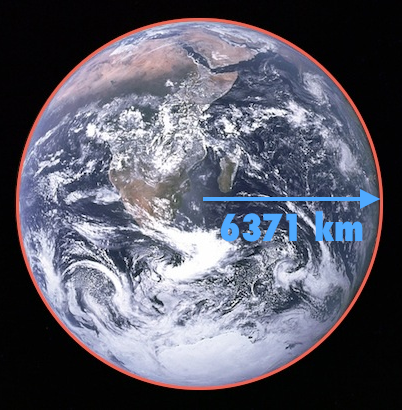
\includegraphics[scale=\shrinkfactor]{figures/b13ca0ce2e95cd21069652083e018a8c654aafe8.png}
\DIFaddend 


\paragraph{Ans} [[? input-number 1]]  $\text{km}$  40030.173592041145

\paragraph{Hint 1}The length of each rope is equal to the circumference of the Earth.

The circumference of a circle with radius $\blue{r}$ is $\red{C}=2\pi \blue{r}$.

We can find the length of the two rope by computing the circumference of a circle of radius $\blue{r}= \blue{6371}\text{ km}$. 

\paragraph{Hint 2}The circumference of a circle with radius $\blue{r}= \blue{6371}\text{ km}$ is

\begin{align*}
\qquad \red{C} 
&=2\pi \blue{r}  \\[2mm]
&=2\pi (\blue{6371}\text{ km}) \\[2mm]
&= 12742\pi \text{ km}.
\end{align*}

\paragraph{Hint 3}The length of the rope is $12742\pi\text{ km}$.



\medskip
\noindent
\textbf{Tags:} {\footnotesize CC.7.G.B.4, SB.7.1.F.2.SR, Area and circumference of a circle.Circle circumference}\\
\textbf{Version:} c1516072.. 2013-10-11
\smallskip\hrule





\section{\href{https://www.khanacademy.org/devadmin/content/items/xb4dd0f0616538444}{xb4dd0f0616538444}}

\noindent
The circumference of a circle $C$ is proportional to the circle's diameter $d$.

**What is the constant of proportionality?**

\paragraph{Ans} $C= $ [[? input-number 1]]$d$   3.141592653589793

\paragraph{Hint 1}This question tests your knowledge of the formula for the circumference of a circle. 

\paragraph{Hint 2}The circumference of a circle with diameter  $\green{d} $ is $\blue{C}=\pi \green{d}$.  The bigger the diameter, the bigger the circumference. 

We can find the constant of proportionality by dividing the circumference by the diameter 

$\qquad \dfrac{\blue{C}}{\green{d}}=\pi$. 



\paragraph{Hint 3}This is how the number $\pi$ is defined.
The number $\pi = 3.14159265\ldots$ is defined as the constant of proportionality which relates the circle's diameter to its circumference**.**




\medskip
\noindent
\textbf{Tags:} {\footnotesize CC.7.G.B.4, SB.7.1.F.2.SR, Area and circumference of a circle.Circle circumference}\\
\textbf{Version:} a1c044c5.. 2013-09-30
\smallskip\hrule





\section{\href{https://www.khanacademy.org/devadmin/content/items/xe55a1e1bf7230020}{xe55a1e1bf7230020}}

\noindent
The figure below shows two ropes that circle around the Earth. The $\red{\text{red}}$ rope hugs the surface of the Earth. The $\purple{\text{purple}}$ rope lies $1\text{ m}$ above the surface of the Earth.

**What is the difference between the lengths of the two ropes?**


\DIFdelbegin \DIFdelend \DIFaddbegin 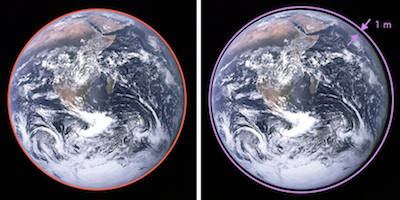
\includegraphics[scale=\shrinkfactor]{figures/02e186d24234a3c609c085669b94c4c7a16ebf33.png}
\DIFaddend 

The  answer to this question does not depend on the radius of the Earth, but in case you wanted to know, the radius of the Earth is approximately $R= 6,371,000\text{ m}$.

\paragraph{Ans} [[? input-number 1]]  $\text{m}$  6.283185307179586

\paragraph{Hint 1}The length of each rope depends on the radius of the circle it makes. 

The circumference of a circle with radius $r$ is $C=2\pi r$.

We can find the difference in the lengths of the two ropes by computing the difference in the circumference of a circle of radius $r=R$ and a circle of radius $r=R+1$, where $R$ represents the radius of the Earth.

\paragraph{Hint 2}The circumference of the $\red{\text{red}}$ rope is 

$\qquad \red{C_1}=2\pi r =2\pi R$.

\paragraph{Hint 3}The circumference of the $\purple{\text{purple}}$ rope is

$\qquad \purple{C_2}=2\pi r =2\pi (R+1)$.

\paragraph{Hint 4}The difference between the circumference of the purple circle and the red circle is

\begin{align*}
\qquad  d 
& = \purple{C_2} - \red{C_1} \\
&= 2\pi (R+1) \ - \ 2\pi R  \\
&= \cancel{2\pi R} + 2\pi \ \cancel{- \ 2\pi R} \\
& = 2\pi
\end{align*} 



\paragraph{Hint 5}The difference in the lengths of the two ropes is $2\pi\text{ m}$.



\medskip
\noindent
\textbf{Tags:} {\footnotesize CC.7.G.B.4, SB.7.1.F.2.SR, Area and circumference of a circle.Circle circumference}\\
\textbf{Version:} 3e3fbdae.. 2013-10-11
\smallskip\hrule





\section{\href{https://www.khanacademy.org/devadmin/content/items/xed9b14030db454cd}{xed9b14030db454cd}}

\noindent
You are standing next to a really big lake which has the shape of a circle. You want to measure the diameter of the lake, but you don't want to have to swim across carrying a meter tape! You decide to walk around the perimeter of the lake and measure its circumference.

**If the circumference is $C=400\pi\text{ m}$, what is the diameter of the lake?**

\paragraph{Ans} $d=$ [[? input-number 1]]  $\text{m}$  400

\paragraph{Hint 1}This problem calls for the formula of the circumference of a circle $\blue{C}=\pi \green{d}$. 

\paragraph{Hint 2}You measured the length of the circumference of the lake to be $\blue{C} =\blue{400\pi}\text{ m}$.

\paragraph{Hint 3}To find the diameter of the lake we must solve for $\green{d}$ in the following equation 

\begin{align*}
  \qquad  \pi \green{d} &= \blue{C} \\[1mm]
\pi \green{d} 	&= \blue{400\pi}\text{ m} \\[1mm]
  \qquad  \cancel{\pi} \green{d} 	
&= 400\cancel{\pi}\text{ m} \\[1mm] 
  \green{d} &= 400\text{ m}
\end{align*}




\medskip
\noindent
\textbf{Tags:} {\footnotesize CC.7.G.B.4, SB.7.1.F.2.SR, Area and circumference of a circle.Circle circumference}\\
\textbf{Version:} 97ded479.. 2013-10-13
\smallskip\hrule





\section{\href{https://www.khanacademy.org/devadmin/content/items/xf0da61cdc2f37004}{xf0da61cdc2f37004}}

\noindent
You are going on a field trip in a school bus. A special detector placed on one of the tires of the school bus measures the number of turns completed by the tire during the journey. The tire's diameter is $1\text{ m}$.

**What is the total distance traveled during the trip, if the tire makes 8000 turns during the trip?**

State \DIFdelbegin \DIFdel{you }\DIFdelend \DIFaddbegin \DIFadd{your }\DIFaddend answer in $\text{km}$.

\paragraph{Ans} [[? input-number 1]]  $\text{km}$  25.132741228718345

\paragraph{Hint 1}Each time the bus wheel rolls forward through one rotation, the bus moves forward a distance equal to the circumference of the tire.

The distance traveled by the bus depends on the number of rotations and the circumference of the tire.

\paragraph{Hint 2}The circumference of a circle with diameter $\green{d}$ is $\blue{C}=\pi \green{d}$.

The bus tire has diameter $\green{d}=\green{1}\text{ m}$ so the circumference of the tire is

\begin{align*}
\qquad \blue{C} &=\pi \green{d} \\
&=\pi( \green{1}) \\
&=\blue{\pi} \text{ m}.
\end{align*}

\paragraph{Hint 3}Since the bus tire makes $\pink{8000}$ turns during the trip, the total distance traveled is $\pink{8000}$ times the circumference of the tire:

\begin{align*}
\qquad \text{distance travaled} 
 & = \pink{8000}\cdot \blue{C} \\ 
 & = \pink{8000}\cdot \blue{\pi}\text{ m} \\
 & = 8000\pi  \text{ m}.
\end{align*}

\paragraph{Hint 4}The total distance traveled during the trip is $8000\pi  \text{ m}$, which is the same as $8\pi  \text{ km}$.



\medskip
\noindent
\textbf{Tags:} {\footnotesize CC.7.G.B.4, SB.7.1.F.2.SR, Area and circumference of a circle.Circle circumference}\\
\textbf{Version:} \DIFdelbegin \DIFdel{cf162f8d.. 2013-10-11
}\DIFdelend \DIFaddbegin \DIFadd{5ae7ad5a.. 2013-10-16
}\DIFaddend \smallskip\hrule





\section{\href{https://www.khanacademy.org/devadmin/content/items/x790eb845d377100f}{x790eb845d377100f}}

\noindent
**Find the area of the shaded region.**


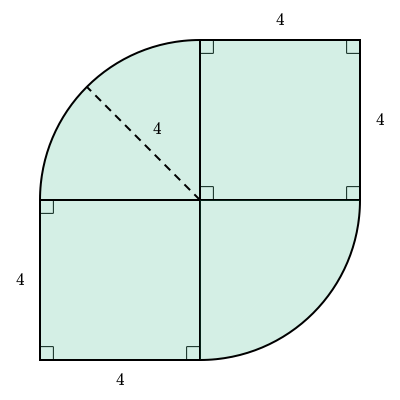
\includegraphics[scale=\shrinkfactor]{figures/eb8635a8059b2c69ad19bf8d44f5a7a7885cf622.png}


\paragraph{Ans} $A =$ 
[[? expression 1]]  32 + 8*pi

\paragraph{Hint 1}The region is a combination of two squares and two quarters of a circle. 
The two squares have side length $\pink{4}$.
The circular sections have radius $\purple{r}=\purple{4}$.

To find the area of the region we can find the area of each of its parts and then add the areas. 

\paragraph{Hint 2}There are two squares in the figure and their total area is 

$\qquad \red{A}=2\times (\pink{4}\times \pink{4}) = \red{32}$.

\paragraph{Hint 3}The circular regions are quarters of a circle. The area of a whole circle is $\pi\purple{r}^2$ so the area of a quarter circle is $\frac{1}{4}$ of $\pi \purple{r}^2$.

The radius of the circular regions is $\red{r}=\red{4}$ and there are $2$ circular parts so their combined area is 

 $\qquad \blue{A} = 2 \times (\frac{1}{4}\pi \purple{r}^2) = \frac{1}{2} \pi \purple{4}^2 = \blue{8\pi}$.


\paragraph{Hint 4}
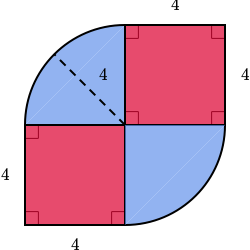
\includegraphics[scale=\shrinkfactor]{figures/be75119c9ec750491ada6dd94f5083c448ab9aad.png} 

The total area of the region is the area of the square parts plus the area of the circular parts:

$\qquad A = \red{32} + \blue{8\pi}$.





\medskip
\noindent
\textbf{Tags:} {\footnotesize CC.7.G.B.4, Area and circumference of a circle.Composite region calculations, SB.7.1.F.2.SR}\\
\textbf{Version:} e99b0573.. 2013-09-30
\smallskip\hrule





\section{\href{https://www.khanacademy.org/devadmin/content/items/x88ec3227d14c19ce}{x88ec3227d14c19ce}}

\noindent
The illustration below shows an office table viewed from above.  

**What is the perimeter of the table?**   

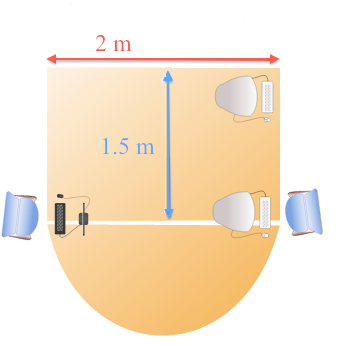
\includegraphics[scale=\shrinkfactor]{figures/2e7c87313a5fdbe0bacdee8a3f8f46418add2f40.png}

Give you answer in $\text{m}$.

\paragraph{Ans} $P=$ 
[[? expression 1]]     5+pi

\paragraph{Hint 1}The table is made up of a rectangular part and a circular part.

We want to find the perimeter of the table. 

Imagine a small insect which walks along the edge of the table. What distance will the insect travel if it makes a full turn around the table and comes back to the point where it started from? 

\paragraph{Hint 2}First let's find the part of the perimeter which is along the rectangular part of the table.

The exterior edge of the rectangular part of the table is

$\qquad P_{\text{rect}} = \blue{1.5}\text{ m} + \red{2}\text{ m} + \blue{1.5}\text{ m}= 5\text{ m}$.

\paragraph{Hint 3}The circular part of the table has the shape of a half-circle with diameter $\red{d}=\red{2}\text{ m}$. The circumference of a circle with dimeter $\red{d}$ is $C=\pi \red{d}$. 

The exterior edge of the circular part of the table is equal to $\purple{\text{half}}$ of the circumference of the full circle:

$\qquad P_{\text{circ}}
= \dfrac{C}{\purple{2}}
= \dfrac{\pi \red{d}}{\purple{2}} 
= \dfrac{\pi (\cancel{\red{2}})}{\cancel{\purple{2}}} 
= \pi \text{ m} $.

\paragraph{Hint 4}The perimeter of the table is the sum of the perimeter of the rectangular and the circular parts of the table:

\begin{align*}
\qquad P_{\text{table}} 
&=  P_{\text{rect}} +  P_{\text{circ}} \\[2mm]
&= 5\text{ m} + \pi \text{ m} \\[2mm]
&= \left( 5 + \pi \right)\text{ m}
\end{align*}

\paragraph{Hint 5}The answer, in $\text{m}$, is therefore $5+\pi$.




\medskip
\noindent
\textbf{Tags:} {\footnotesize CC.7.G.B.4, Area and circumference of a circle.Composite region calculations, SB.7.1.F.2.SR}\\
\textbf{Version:} 85b3454c.. 2013-10-11
\smallskip\hrule





\section{\href{https://www.khanacademy.org/devadmin/content/items/xade69580de9f3c4e}{xade69580de9f3c4e}}

\noindent
**Find the area of the shaded region.**


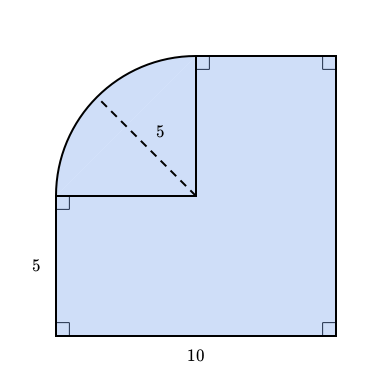
\includegraphics[scale=\shrinkfactor]{figures/b0216381822fdf828c9b1c0c60a3da3a18cdb9da.png}


\paragraph{Ans} $A =$ 
[[? expression 1]]  75 + 25*pi/4

\paragraph{Hint 1}The region in the figure is a combination of an $L$-shaped polygon with right angles and a quarter circle.  The quarter circle has radius $r=5$.

To find the total area of the region we can split it up into parts and then add the areas of the parts.

\paragraph{Hint 2}The curved part is a quarter circle. The area of a whole circle is $\pi r^2$. The area of quarter circle is therefore $\frac{1}{4}$ of $\pi r^2$.

The radius of the circular regions is $r=5$ so the area of a quarter circle is

\begin{align*} 
\qquad \green{A} &= \frac{1}{4}\pi r^2 \\[1mm]
&= \frac{1}{4} \pi 5^2 \\[2mm]
&= \green{\dfrac{25\pi}{4}}\,.
\end{align*}


\paragraph{Hint 3}We can decompose the rest of the region into a rectangle and a square.    

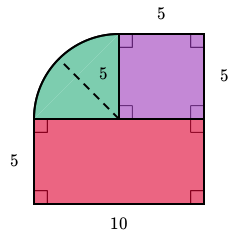
\includegraphics[scale=\shrinkfactor]{figures/5505e58c694464279f963187f09c2f77d54a9a63.png} 

First calculate the are area of the rectangular region:
The area of this rectangular region is 

$\qquad \red{A}=5\times 10 = \red{50}$.

Next we calculate the area of the square region.
The square has side length $5$ so the its area is  

$\qquad \purple{A}=5\times 5 = \purple{25}$.


\paragraph{Hint 4}The total area of the region is the sum of the area of the $\green{\text{quarter circle}}$, the area of the $\red{\text{rectangular region}}$, and area of the $\purple{\text{square region}}$:

\begin{align*}
\qquad A &= \green{\dfrac{25\pi}{4}} + \red{50} + \purple{25}\\ &=  \dfrac{25\pi}{4}+ 75.
\end{align*}

The total area of the shaded region is $A=\dfrac{25\pi}{4}+ 75$.



\medskip
\noindent
\textbf{Tags:} {\footnotesize CC.7.G.B.4, Area and circumference of a circle.Composite region calculations, SB.7.1.F.2.SR}\\
\textbf{Version:} 0093daff.. 2013-10-09
\smallskip\hrule





\section{\href{https://www.khanacademy.org/devadmin/content/items/xae170cfcb857d9e1}{xae170cfcb857d9e1}}

\noindent
**Find the perimeter of the shaded region.**


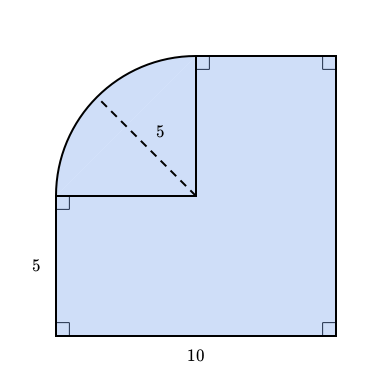
\includegraphics[scale=\shrinkfactor]{figures/b0216381822fdf828c9b1c0c60a3da3a18cdb9da.png}

\paragraph{Ans} $P =$ 
[[? expression 1]]  30 + 5*pi/2

\paragraph{Hint 1}The region in the figure is a combination of an $L$-shaped polygon with right angles and a quarter circle.  The quarter circle has radius $r=5$.

To find the perimeter of the region we can split its boundary into two parts and then add the lengths of the two parts.

\paragraph{Hint 2}The curved part is a quarter circle. The circumference of a whole circle is $2\pi r$. The length of quarter circle is therefore $\frac{1}{4}$ of $2\pi r$.

The radius of the circular regions is $r=5$ so the length of the edge of the quarter circle is

\DIFdelbegin \begin{eqnarray*}\DIFdel{ 
\qquad \green{P_1} }&\DIFdel{= \frac{1}{4}2\pi r }\\[1mm]
&\DIFdel{= \frac{1}{2} \pi 5 }\\[2mm]
&\DIFdel{= \green{\dfrac{5\pi}{2}}\,.
}\end{eqnarray*}
\DIFdelend \DIFaddbegin \begin{align*}\DIFadd{ 
\qquad \green{P_1} }&\DIFadd{= \frac{1}{4}2\pi r }\\[1mm]
&\DIFadd{= \frac{1}{2} \pi 5 }\\[2mm]
&\DIFadd{= \green{\dfrac{5\pi}{2}}\,
}\end{align*}
\DIFaddend 


\paragraph{Hint 3}We rest of the perimeter of the region consists of straight lines.

Starting from the top center of the figure and going around the region in the clockwise direction we see the following lengths:

$\qquad \red{P_2}=5 +  10 +10 +5 = \red{30}$.

\paragraph{Hint 4}The perimeter of the region is the sum of the length of the $\green{\text{circular}}$ part and the length  of the $\red{\text{straight}}$ lines:

\begin{align*}
\qquad P &=  \green{P_1} + \red{P_2} = \green{\dfrac{5\pi}{2}} + \red{30}.
\end{align*}

The total perimeter of the shaded region is $P=\dfrac{5\pi}{2}+ 30$.



\medskip
\noindent
\textbf{Tags:} {\footnotesize CC.7.G.B.4, Area and circumference of a circle.Composite region calculations, SB.7.1.F.2.SR}\\
\textbf{Version:} \DIFdelbegin \DIFdel{62b5cd1f.. 2013-10-15
}\DIFdelend \DIFaddbegin \DIFadd{4d7913ea.. 2013-10-16
}\DIFaddend \smallskip\hrule





\section{\href{https://www.khanacademy.org/devadmin/content/items/xe76e25d5bcae424a}{xe76e25d5bcae424a}}

\noindent
The illustration below shows an office table viewed from above.  

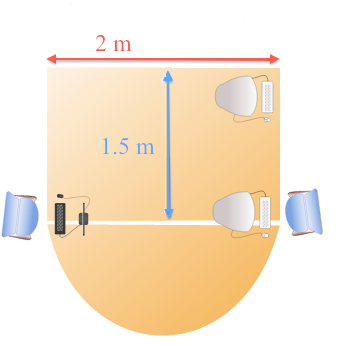
\includegraphics[scale=\shrinkfactor]{figures/2e7c87313a5fdbe0bacdee8a3f8f46418add2f40.png}

**What is the total area of the table?**  

Give you answer in $\text{m}^2$.

\paragraph{Ans} $A=$ 
[[? expression 1]]  3+pi/2

\paragraph{Hint 1}The total area of the table is equal to the area of the rectangular part of the table plus the area of the circular part.

\paragraph{Hint 2}The area of a rectangular part is equal to its width times  its height $A=\red{w}\times \blue{h}$. 

The rectangular part of the table has area 

$\qquad A = \red{2}\text{ m} \times \blue{1.5}\text{ m} = 3\text{ m}^2$

\paragraph{Hint 3}The circular part of the table has the shape of a half-circle with diameter $\red{d}=\red{2}\text{ m}$. If the diameter of a circle is $\red{d}=\red{2}\text{ m}$ then its radius is $\green{r}=\green{1}\text{ m}$ and its area is $A=\pi \green{r}^2=\pi\text{ m}^2$.

The area of the circular part of the table is equal to $\purple{\text{half}}$ of the area of the full circle:

$\qquad A 
= \purple{\dfrac{1}{2}}\pi\green{r}^2
= \purple{\dfrac{1}{2}}\pi(\green{1})^2
= \dfrac{\pi}{2}\text{ m}^2 $



\paragraph{Hint 4}The total area of the table is the sum of the areas of the  rectangular and the circular parts of the table:

\begin{align*}
\qquad A_{\text{table}} 
&= 3\text{ m}^2 + \dfrac{\pi}{2} \text{ m}^2 \\
&= \left(3+\dfrac{\pi}{2}\right)\text{ m}^2
\end{align*}

\paragraph{Hint 5}The answer, in $\text{m}^2$, is therefore $3+\dfrac{\pi}{2}$.




\medskip
\noindent
\textbf{Tags:} {\footnotesize CC.7.G.B.4, Area and circumference of a circle.Composite region calculations, SB.7.1.F.2.SR}\\
\textbf{Version:} cc261381.. 2013-10-09
\smallskip\hrule





\section{\href{https://www.khanacademy.org/devadmin/content/items/xefc631c99946d20d}{xefc631c99946d20d}}

\noindent
**Find the area of the shaded region.**


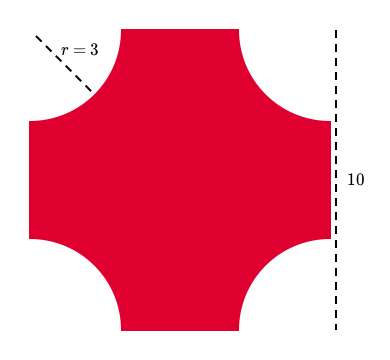
\includegraphics[scale=\shrinkfactor]{figures/ec1d9546c0b030bf9e41bb394bf1c4337b8a1c2c.png}

\paragraph{Ans} $A =$ 
[[? expression 1]]  100-9*pi

\paragraph{Hint 1}The area of the shaded region looks like a square with the four corners cut out. Each of the corners is one quarter of a circle. Thus, to find the area of the shaded region we can find the area of the square and subtract the area that is missing from the four corners.

\paragraph{Hint 2}The area of the square (including the corners) is   

$\qquad \purple{A}=10\times 10 = \purple{100}$.

\paragraph{Hint 3}Each of the corners is a quarter circle with radius $\red{r}=\red{3}$, and there are four corners so the total area that is missing is equal to the area of one whole circle with radius $\red{r}=\red{3}$.
The area of a circle of radius $\red{3}$ is 

 $\qquad \blue{A} = \pi (\red{r})^2 = \pi \red{3}^2 = \blue{9\pi}$.

\paragraph{Hint 4}Therefore, the area of the shaded region is equal to $\purple{100} - \blue{9\pi}$.



\medskip
\noindent
\textbf{Tags:} {\footnotesize CC.7.G.B.4, Area and circumference of a circle.Composite region calculations, SB.7.1.F.2.SR}\\
\textbf{Version:} 6154c60c.. 2013-10-09
\smallskip\hrule





\section{\href{https://www.khanacademy.org/devadmin/content/items/xf0fdfd7428fcd860}{xf0fdfd7428fcd860}}

\noindent
**Find the perimeter of the shaded region.**


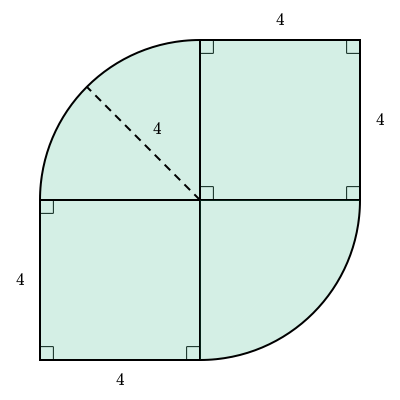
\includegraphics[scale=\shrinkfactor]{figures/eb8635a8059b2c69ad19bf8d44f5a7a7885cf622.png}


\paragraph{Ans} $P =$ 
[[? expression 1]]  16+4*pi

\paragraph{Hint 1}The region is a combination of two squares and two quarters of a circle. 
The two squares have side length $\pink{4}$.
The circular sections have radius $\purple{r}=\purple{4}$.

To find the perimeter of the region we can find the length of the exterior border of each of its parts and then add the lengths. 

\paragraph{Hint 2}The outer borders of the two squares in the figure has a total length of  

$\qquad \red{P_1}=2\times (\pink{4} + \pink{4}) = \red{16}$.

\paragraph{Hint 3}The circular regions are quarters of a circle. The circumference of a whole circle is $2\pi\purple{r}$. The length of a quarter circle is equal to $\frac{1}{4}$ of $2\pi \purple{r}$.

The radius of the circular regions is $\red{r}=\red{4}$ and there are $\green{2}$ of these quarters-circles.
Their combined length of the circular parts is 

\begin{align*}
\qquad \blue{P_2} 
&= \green{2} \times \left(\frac{1}{4}2\pi \purple{r}\right)  \\[2mm]
 &= \green{2} \times \left(\frac{1}{4}2\pi (\purple{4})\right)  \\[2mm]
 &= \green{2} \times \left(\frac{1}{\cancel{4}}2\pi (\cancel{4})\right)  \\[2mm]
&= \blue{4\pi}\text{ m}.
\end{align*}


\paragraph{Hint 4}The total perimeter of the region is the lengths of the exterior borders of the two square parts plus the length  of the circular parts:

$\qquad P = \red{16} + \blue{4\pi}$.





\medskip
\noindent
\textbf{Tags:} {\footnotesize CC.7.G.B.4, Area and circumference of a circle.Composite region calculations, SB.7.1.F.2.SR}\\
\textbf{Version:} b8a0a78a.. 2013-10-13
\smallskip\hrule





\section{\href{https://www.khanacademy.org/devadmin/content/items/x1f4b934dfe143abf}{x1f4b934dfe143abf}}

\noindent
A circle with diameter $d=6$ is cut into twelve slices. The slices are then rearranged so that half of the slices point downward and half point upward so they form a shape that resembles a parallelogram. Since the circle and the parallelogram are made up of the same slices, the area of the two figures is the same.


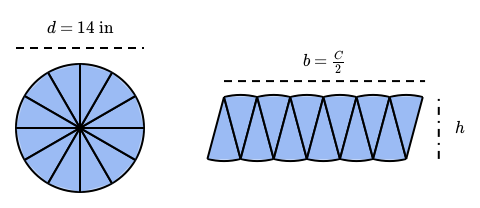
\includegraphics[scale=\shrinkfactor]{figures/fce0c8a558ebd29517b2875384c02ac6b3677f18.png}

The radius of the circle is $r=$ [[? input-number 1]].  
Since the slices come from the circle, the height of the bumpy parallelogram is $h=$ [[? input-number 2]].  
The circumference of the circle is given by the formula $C=2\pi r$. Half the edges of the slices form the base of the parallelogram so the length of the base is equal to half the circumference $b=$ [[? input-number 3]].   
Using the formula for the area of a parallelogram, we find the area of the circle is equal to $A=b\times h=$ [[? input-number 4]].


\paragraph{Ans} Complete the sentences. 

\paragraph{Hint 1}In this exercise we'll use the formula for the circumference of a circle $\blue{C}=2\pi \red{r}$ and some geometry to find the area of a circle.

\paragraph{Hint 2}The circle has diameter $\green{d}=\green{6}$ so its radius is $\red{r}=\frac{\green{d}}{2}=\red{3}$. 

\paragraph{Hint 3}The height of the parallelogram is equal to the length of the slices. Since the slices come from the circle with radius $\red{r}=\red{3}$, the height of the parallelogram is $h=3$.

\paragraph{Hint 4}The circumference of a circle with radius $\red{r}=\red{3}$ is $\blue{C}=2\pi \red{r}=2\pi (\red{3})=\blue{6\pi}$. This corresponds to the length of the edge of the circle. 

When we rearrange the slices in the parallelogram shape, the length of the base of the parallelogram is equal to half of the circumference of the circle:

$\qquad b = \dfrac{\blue{C}}{2} = \dfrac{ \blue{6 \pi}  }{2} = 3\pi$.


\paragraph{Hint 5}The area of the circle is the same as the area of the parallelogram. We can therefore find the area of the circle using the formula for the area of a parallelogram:

$\qquad A=b\times h=3\pi \times 3= 9\pi$.



\medskip
\noindent
\textbf{Tags:} {\footnotesize CC.7.G.B.4, SB.7.1.F.2.SR, Area and circumference of a circle.derive A formula from C formula}\\
\textbf{Version:} 01b2fbf2.. 2013-10-15
\smallskip\hrule





\section{\href{https://www.khanacademy.org/devadmin/content/items/x9a3db47ccf936b4a}{x9a3db47ccf936b4a}}

\noindent
A pizza of radius $r$, diameter $d=2r$, and circumference $2\pi r$ is cut into $12$ slices. The slices are then placed so they form a shape that resembles a parallelogram. Since the circle and the parallelogram are made up of the same slices, the area of the two figures is the same.


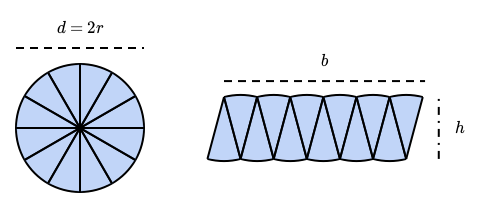
\includegraphics[scale=\shrinkfactor]{figures/3f15087165055ef8a63a60583da95a017c9259b9.png}

In the new arrangement of the slices, the crust of the pizza forms the bottom and top edges of the parallelogram. The length of the base of the parallelogram is equal to half of the circumference of the pizza $b=$ [[? dropdown 1]].  
The height $h$ of the parallelogram is equal to the lengths of the pizza slices $h=$ [[? dropdown 2]].  
Using the formula for the area of a parallelogram $A=b\times h$, we find the area of the pizza is equal to $A=$ [[? dropdown 3]].

\paragraph{Ans} Complete the sentences. 

\paragraph{Hint 1}In this problem we'll use the formula for the circumference of a circle $\blue{C}=2\pi \red{r}$ to derive the formula for the area of a circle $\purple{A}=\pi \red{r}^2$.

\paragraph{Hint 2}We know the circumference of a circle of radius $\red{r}$ is $\blue{C}=2\pi \red{r}$. The total length of the crust of a pizza with radius $\red{r}$ is $2\pi \red{r}$.

When we rearrange the slices in the parallelogram shape, the length of the base of the parallelogram is equal to half of the circumference of the pizza:

$\qquad b = \dfrac{\blue{C}}{2} = \dfrac{ 2 \pi \red{r} }{2} = \pi \red{r}$.

\paragraph{Hint 3}The height of the parallelogram is equal to the length of the pizza slices. Since the slices come from a pizza with radius $\red{r}$, the length of each pizza slice is $\red{r}$. Thus, the height of the parallelogram is $h=\red{r}$.

\paragraph{Hint 4}The area of the pizza is the same as the area of the parallelogram. We can therefore find the area of the pizza by using the formula for the area of a parallelogram $A=b\times h=\pi\red{r}\times \red{r}=\pi \red{r}^2$.

\paragraph{Hint 5}The length of the base of the parallelogram is $b=\pi\red{r}$. The height $h$ of the parallelogram is  $h= \red{r}$. The area of the pizza is equal to $A=\pi \red{r}^2$.



\medskip
\noindent
\textbf{Tags:} {\footnotesize CC.7.G.B.4, SB.7.1.F.2.SR, Area and circumference of a circle.derive A formula from C formula}\\
\textbf{Version:} b5b399fc.. 2013-10-09
\smallskip\hrule





\section{\href{https://www.khanacademy.org/devadmin/content/items/xb9d0da8f1cff505a}{xb9d0da8f1cff505a}}

\noindent
Lucy wants to calculate the area of a $14\text{ in}$ pizza, but she forgot the formula for the area of a circle. She decides to cut the pizza into slices and rearrange the slices so that half the slices point downward and half point upward to form a parallelogram. Since the pizza-circle and the pizza-parallelogram are made up of the same slices, the area of the pizza is the same as the area of the parallelogram.


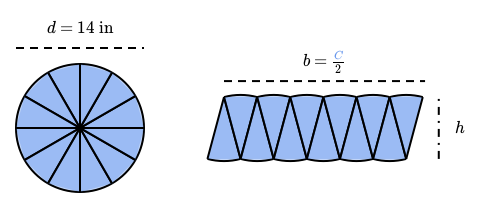
\includegraphics[scale=\shrinkfactor]{figures/26c47c40d180b9cf4072b9fd7b879e8d39d5d86a.png}

Since the slices come from the pizza, the height of the bumpy parallelogram is equal to the radius of the pizza  $h=r=$ [[? input-number 1]] $\text{ in}$.  
The length of the base of the parallelogram is equal to half of the circumference of the pizza $b=\frac{C}{2}=$  [[? input-number 2]]$\text{ in}$.  
The area of a parallelogram is equal to the length of its base times its height $A=b\times h$. The area of the pizza is therefore $A=$ [[? input-number 3]] $\text{in}^2$. 

\paragraph{Ans} Complete the sentences. 

\paragraph{Hint 1}In this exercise we will use the formula for the area of a parallelogram $A=b\times h$ and the formula for the circumference of a circle $C=2\pi r$ to find the area of the pizza.

\paragraph{Hint 2}The height of the parallelogram is equal to the radius  of the pizza. Thus, the height of the parallelogram is $h=r=7\text{ in}$.

\paragraph{Hint 3}We know the circumference of a circle of radius $r$ is $C=2\pi r$. The total length of the crust of a pizza with radius $r$ is $2\pi r$. When we rearrange the slices in the parallelogram shape, the length of the base of the parallelogram is equal to half of the circumference of the pizza:

$\qquad b = \dfrac{C}{2} = \dfrac{ 2 \pi r }{2}= \pi r=7\pi\text{ in}$.


\paragraph{Hint 4}The area of a parallelogram is equal to the length of its base times its heights $A=b\times h$.

The length of the base of the parallelogram is $b=7\pi\text{ in}$ and its height is $h=7\text{ in}$, therefore its area is 

$\qquad A= b \times h = 7\pi\text{ in}\times 7\text{ in} = 49\pi\text{ in}^2$.


\paragraph{Hint 5}Since the circle and the parallelogram have the same are, the area of the pizza is $49\pi\text{ in}^2$.




\medskip
\noindent
\textbf{Tags:} {\footnotesize CC.7.G.B.4, SB.7.1.F.2.SR, Area and circumference of a circle.derive A formula from C formula}\\
\textbf{Version:} 3afa31d4.. 2013-10-15
\smallskip\hrule





\end{document}

